
% !TEX TS-program = pdflatex
\documentclass[12pt,a4paper]{article}
\usepackage{amsmath,amssymb,siunitx,graphicx,booktabs,listings,hyperref}
\usepackage{caption}
\usepackage{subcaption}
\usepackage{geometry}
\geometry{margin=1in}
\usepackage{titlesec}
\usepackage{titling}
\usepackage{fancyhdr}
\usepackage{lastpage}

% Define placeholders for key results
\newcommand{\MaxScale}{\textbf{0.6234}}%
\newcommand{\PzeroOne}{\textbf{206.53}}%
\newcommand{\PzeroTwo}{\textbf{250.00}}%
\newcommand{\CompPointP}{\textbf{1.2105}}%
\newcommand{\CompPointM}{\textbf{10.5503}}%

% Create a title page style
\makeatletter
\renewcommand{\maketitle}{%
  \begin{center}
    \vspace*{4cm}
    \LARGE\textbf{ME302 : 2024-25 - II} \\[1cm]
    \LARGE\textbf{Course Project Report} \\[4cm]
    \large
    Akshit Shukrawal (220107) \\
    Dharmendra Jangir (220353) \\
    Harsh Singh (220434) \\[2cm]
    \large April 15, 2025
  \end{center}
  \thispagestyle{empty}
  \newpage
}
\makeatother

\begin{document}

% Just the title page
\maketitle

\section*{Problem Description}
A turbomachine component designed for a future gas turbine engine (prototype characteristic length $\ell_{\mathrm{prototype}}=0.2\,\mathrm{m}$) is to be tested at a reduced scale in a closed-loop high-pressure facility. The objective is to determine the maximum geometric scale $S=\ell_{\mathrm{model}}/\ell_{\mathrm{prototype}}$ (with $0<S<1$) such that both Mach number ($M=0.55$) and Reynolds number ($Re=3.0\times10^6$ based on $\ell$) similarity are maintained, while satisfying facility constraints:
\begin{enumerate}
  \item Maximum allowable stagnation pressure anywhere: $P_{0i}\leq250\,\mathrm{kPa}$.
  \item Outlet chamber pressure $P_{05}\geq P_{01}$ to sustain closed-loop operation.
\end{enumerate}
Inlet stagnation temperature is fixed at $T_{01}=293\,\mathrm{K}$.  The test-section inlet diameter $D_4=2\,\ell_{\mathrm{model}}$.  Stagnation losses are 1.5\% from station 2 to 3, and 5\% from station 4 to 5.  Air is assumed ideal ($R=287\,\mathrm{J/kg\,K}$, $\gamma=1.4$) with viscosity $\mu=1.83\times10^{-5}\,\mathrm{Pa\,s}$.  Compressor map data ($\dot m_{\mathrm{ref}}$, $T_0$ ratio, $P_0$ ratio) are provided in the supplementary spreadsheet.\\
\section*{Part (a): Geometric Scaling Analysis}

\section*{Methodology}
We adopt an analytical–computational approach, implemented in Python, to sweep compressor operating points and inlet pressures, enforcing similarity and constraints.  The procedure is as follows:

\subsection*{Solution Algorithm}
Initialize a variable $\mathit{maxscale} = 0$. This variable stores the largest possible scale value with the given setup, and is updated after every iteration.\\
We start with initializing $P_{01}$ with the largest possible value ($P_{01} = 250\,\mathrm{kPa}$), and update it after every iteration.

Then we start the computation loop for all the points in the dataset.\\
Mass flow at station 4 ($T_{01}=293\,\mathrm{K}$) :
\begin{align}
  \dot{m}
    &= \dot{m}_{\mathrm{ref}} \left(\frac{P_{01}}{101.325\,\mathrm{kPa}}\right)
             \sqrt{\frac{293\,\mathrm{K}}{T_{01}}} \nonumber \\
    &= \dot{m}_{\mathrm{ref}} \left(\frac{P_{01}}{101.325\,\mathrm{kPa}}\right) \times 1
\end{align}
Substituting the value of $P_{01}$ in Eq.~(1) gives the value of $\dot{m}$.

But,
\begin{align}
  \dot{m} &= \rho_4 A_4 c_4 \nonumber \\
          &= \rho_4 \left(\frac{\pi d^2}{4}\right) c_4 \nonumber \\
          &= \rho_4 \left(\frac{\pi (2 l_{\mathrm{model}})^2}{4}\right) c_4 \nonumber \\
          &= (\rho_4 c_4) \pi l_{\mathrm{model}}^2
\end{align}

Also,
\begin{align}
  Re &= \frac{\rho_4 c_4 l_{\mathrm{model}}}{\mu_4} = \frac{\rho_4 c_4 l_{\mathrm{model}}}{\mu} \nonumber \\
  \Rightarrow \rho_4 c_4 &= \frac{Re\, \mu}{l_{\mathrm{model}}}
\end{align}

Substituting the value of $\rho_4 c_4$ from Eq.~(3) in Eq.~(2) :
\begin{align}
  \dot{m} &= \left(\frac{Re\, \mu}{l_{\mathrm{model}}}\right) \pi l_{\mathrm{model}}^2 \nonumber \\
          &= Re\, \mu\, \pi\, l_{\mathrm{model}} \nonumber \\
  \Rightarrow l_{\mathrm{model}} &= \frac{\dot{m}}{Re\, \mu\, \pi}
\end{align}

Since the Reynolds number is kept constant in scaling ($Re = 3.0 \times 10^6$), substituting the values of $Re$ and $\mu$ in Eq.~(5), we will get the corresponding value of $l_{\mathrm{model}}$.\\

Thus, the scale :
\begin{align}
S = \frac{l_{\mathrm{model}}}{l_{\mathrm{prototype}}} = \frac{l_{\mathrm{model}}}{0.2\,\mathrm{m}}
\end{align}

Stagnation properties at compressor exit (station 2) relate to inlet $P_{01}$ via the compressor map :
\begin{align}
  P_{02} &= (P_0\mathrm{ratio})\,P_{01}\\
  T_{02} &= (T_0\mathrm{ratio})\,T_{01}
\end{align}
Solving Eq.~(6) and (7), we get corresponding $P_{02}$ and $T_{02}$.\\
Pressure losses give :
\begin{align}
  P_{03} &= (1-0.015)\,P_{02}\\
  P_{05} &= (1-0.05)\,P_{04}
\end{align}
By substituting the value of $P_{02}$ in Eq.~(8), we get corresponding value of $P_{03}$.\\
Now, since the system is adiabatic beyond station 2, we take $T_{02} = T_{03} = T_{04}$.\\
Now, the Mach number is also constant while scaling ($M = 0.55$). So, we find $T_{4}$ from :
\begin{align}
\frac{T_{04}}{T_4} &= 1 + \frac{\gamma - 1}{2} M^2 \nonumber \\
\Rightarrow T_4 &= \frac{T_{04}}{1 + \frac{\gamma - 1}{2} M^2}
\end{align}
But, Mach number can also be written as :
\begin{align}
M &= \frac{c_4}{\sqrt{\gamma R T_4}} \nonumber \\
\Rightarrow c_4 &= M \sqrt{\gamma R T_4}
\end{align}
which gives us $c_{4}$.\\
Rearranging Eq.~(3), we get :
\begin{align}
  \rho_4 &= \frac{Re\, \mu}{c_4 l_{\mathrm{model}}}
\end{align}
Now, substituting $l_{model}$, $Re$ and $c_{4}$ in Eq.~(12), we get the value of $\rho_{4}$.\\
Now, considering ideal gas behaviour :
\begin{align}
  P_4 &= \rho_4 R T_4
\end{align}
Substituting the values of $rho_{4}$ and $T_{4}$ in Eq.~(13) gives the pressure $P_{4}$.\\
Now, the relation between stagnation and static conditions is the adiabatic relationship :
\begin{align}
P_4^{1-\gamma}T_4^\gamma &= P_{04}^{1-\gamma}T_{04}^\gamma \nonumber \\
\Rightarrow P_{04} &= P_4 \left(\frac{T_4}{T_{04}}\right)^{\frac{\gamma}{1-\gamma}}
\end{align}
Substituting the values of $P_{4}$, $T_{4}$ and $T_{04}$ in Eq.~(14) gives $P_{04}$.\\
Now, $P_{05}$ was found from Eq.~(9), using the value of $P_{04}$ derived above.\\
Check if all the design constraints are satisfied, i.e., $P_{01} \leq P_{05}$ and $P_{01}, P_{02}, P_{03}, P_{04}, P_{05} \leq 250\,\mathrm{kPa}$.\\

If all the constraints are satisfied, update $\mathit{maxscale} = \mathit{scale}$ if $\mathit{scale} > \mathit{maxscale}$, and remember the corresponding $P_0$ ratio, $T_0$ ratio, and $\dot{m}_{\mathrm{ref}}$.\\

Now reduce $P_{01}$ by $0.001$ (or any other suitable value depending on the accuracy required), and repeat the loop.\\
Keep running the loop until either:
\begin{itemize}
    \item There is no suitable point in the dataset ($\mathit{maxscale}$ is not updated), or
    \item $P_{01}$ becomes zero (vacuum condition)
\end{itemize}

\subsection*{Additional Steps for Optimization}

\subsubsection*{1. Static Pressure Safety Margin}
While the facility's structural limit is specified for stagnation pressures ($P_{0i} \leq 250\,\mathrm{kPa}$), we recognize that the actual wall loading depends on \textit{static pressures} ($P_i$), which are always lower than stagnation pressures.\\
For additional optimization, at station 3, we apply the isentropic mass flow rate equation :
\begin{align}
\frac{\dot{m} \sqrt{C_p T_{03}}}{A_n P_{03}} 
= \frac{\gamma}{\sqrt{\gamma - 1}} \cdot 
\frac{M_3}{\left(1 + \frac{\gamma - 1}{2} M_3^2 \right)^{\frac{\gamma + 1}{2(\gamma - 1)}}}
\end{align}
We have
\begin{align}
A_n = \frac{\pi D^2}{4}, \quad \text{where } D = 0.6\,m
\end{align}
Thus, in Eq.~(15), $\dot{m}$, $C_p$, $T_{03}$, $P_{03}$, $A_n$ and $\gamma=1.4$ are known.\\
So, the resulting equation would be a 6 degree polynomial, whose roots will give the Mach number ($M_3$) at station 3 (we will only consider the roots greater than 0.55, as it is an upstream diffuser, so $M_3 > M_4$).\\
This equation can be solved using numerical methods in Python using specific libraries.\\
Once we get $M_3$, we can calculate the static pressure $P_3$ using the formula :
\begin{align}
\frac{P_3}{P_{03}} = \left( 1 + \frac{\gamma - 1}{2} M_3^2 \right)^{-\frac{\gamma}{\gamma - 1}} \nonumber \\
\Rightarrow \quad P_3 = P_{03} \left( 1 + \frac{\gamma - 1}{2} M_3^2 \right)^{-\frac{\gamma}{\gamma - 1}}
\end{align}

Similarly, we can calculate $P_1$, $P_2$, $P_3$ and $P_5$.\\
Now we can apply the pressure constraints $P_{01} \leq P_{05}$ and $P_{1}, P_{2}, P_{3}, P_{4}, P_{5} \leq 250\,\mathrm{kPa}$, and proceed the computation as before.\\
This method would disregard additional safety margins, and any excess pressure above these values might lead to failure of the apparatus.

\subsubsection*{2. Dataset Extrapolation}
The provided compressor map has finite data points. To find the absolute maximum scale:
\begin{itemize}
  \item Fit a curve to the compressor map's $P_0$ ratio vs. $\dot{m}_{\mathrm{ref}}$ data.
  \item Extrapolate to higher mass flow rates while maintaining $P_{05} \geq P_{01}$.
  \item The theoretical maximum occurs when:
    \[
    \frac{P_{05}}{P_{01}} = 0.95 \times 0.985 \times P_0\,\mathrm{ratio} \geq 1 \implies P_0\mathrm{ratio} \geq 1.0687
    \]
\end{itemize}


\section*{Results}

The maximum allowable scale is found to be \(\mathbf{0.62333}\).  
The corresponding inlet stagnation pressure is \(\mathbf{206.500}\,\boldsymbol{\mathrm{kPa}}\), yielding compressor exit stagnation pressure \(\mathbf{249.959}\,\boldsymbol{\mathrm{kPa}}\).\\
The selected operating point on the compressor map is at \(\mathbf{P_0}\) \textbf{ratio = }\(\mathbf{1.210454}\) and \(\boldsymbol{\dot{m}_{\mathrm{ref}}} = \mathbf{10.550284}\,\boldsymbol{\mathrm{kg/s}}\).

\begin{figure}[h!]
  \centering
  \fbox{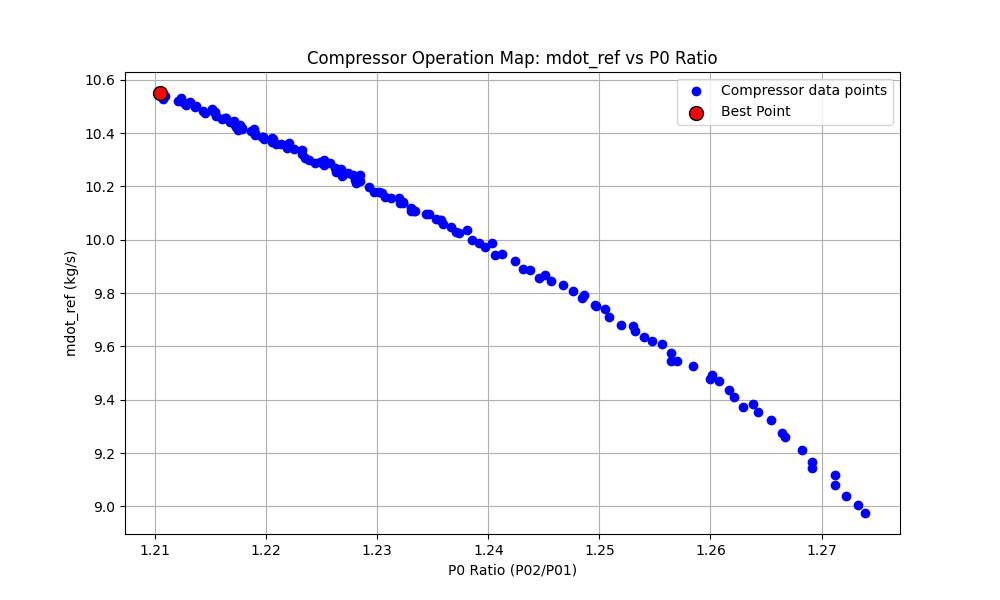
\includegraphics[width=0.8\textwidth]{Compressor_map_best_point.png}}
  \caption{Compressor map showing the selected operating point.}
  \label{fig:compressor_map}
\end{figure}

\begin{figure}[h!]
  \centering
  \fbox{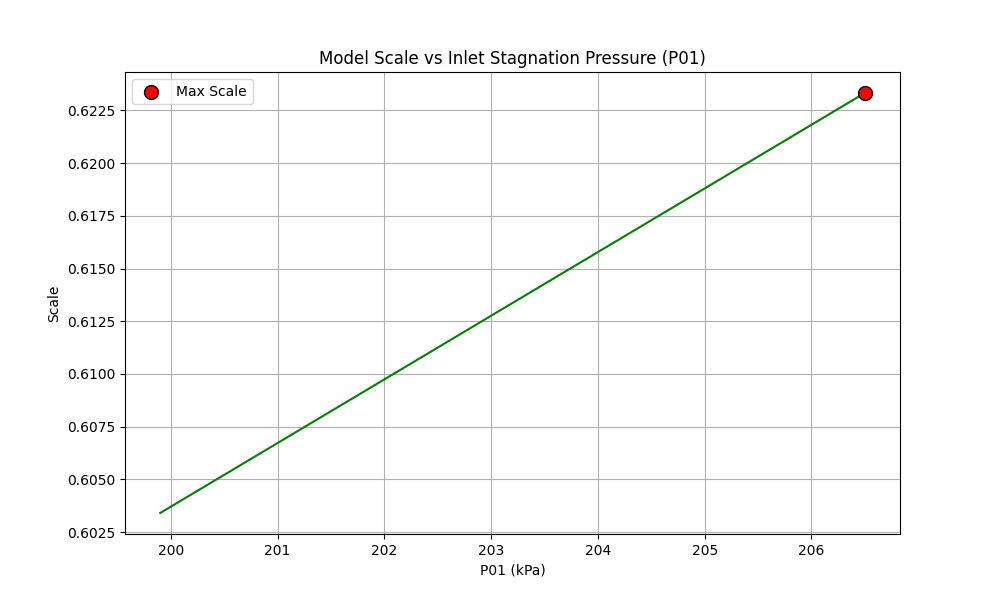
\includegraphics[width=0.8\textwidth]{Scale_vs_P01.png}}
  \caption{Scale \(S\) as a function of inlet stagnation pressure \(P_{01}\).}
  \label{fig:scale_curve}
\end{figure}


\clearpage

% ================ Part (b): Experimental Research Studies ================
\section*{Future Work}
\section*{Part (b): Experimental Research Studies}

Part (b) of the problem is divided into three parts. Each part provide a comprehensive view of experimental research studies aimed at modifying the test section and upstream diffuser along with the technological objectives, benefits and applications, and the industrial sponsors that might be interested in supporting the research. Each study focuses on different aspects—from passive geometric optimization to advanced active control—with direct implications for enhancing engine performance, fuel efficiency, and overall reliability. These studies hold significant promise for innovation in aerospace propulsion, with wide-ranging industrial applications and sponsorship prospects.


% Note: The following Part (b) content has been integrated with the same LaTeX styling as Part (a).

\subsection*{(i): Diffuser Geometry Optimization and Passive Flow Control}


\textbf{Experimental Concept:}\\[0.5em]
This study focuses on redesigning the upstream diffuser by incorporating adjustable geometry features. For instance, the diffuser walls could be made movable or hinged to vary the diffuser semi-angle and throat area, thereby allowing systematic control over the flow expansion process. In the test section, high-resolution pressure taps and optical diagnostics (such as Particle Image Velocimetry, PIV) will capture detailed information on flow separation, wake formation, and total pressure recovery under various diffuser configurations.

\vspace{0.5em}
\begin{figure}[h!]
  \centering
  \fbox{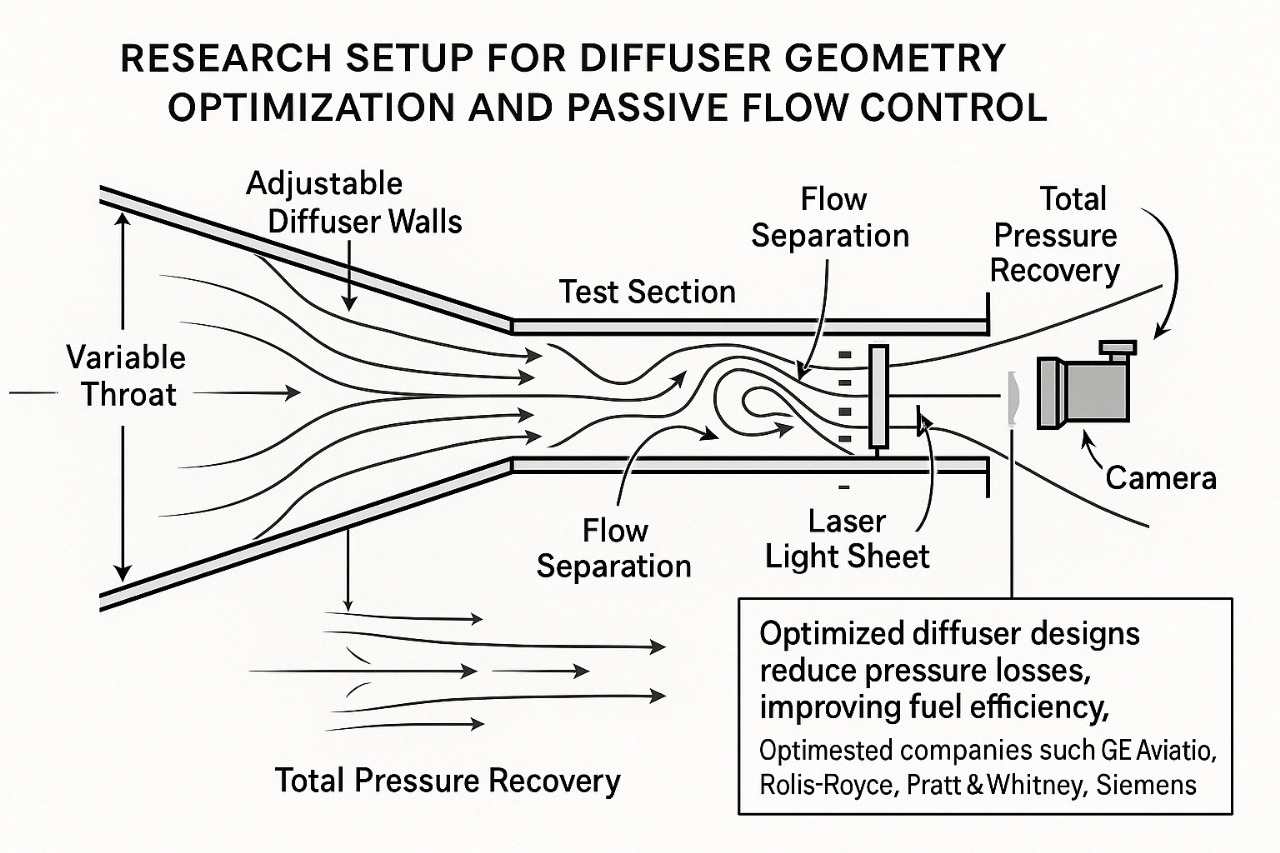
\includegraphics[width=0.8\textwidth]{Diffuser geometry.jpg}}
  \caption{Compressor map showing the selected operating point.}
  \label{fig:compressor_map}
\end{figure}

\vspace{0.5em}
\textbf{Technological Advancement \& Industrial Appeal:}\\[0.5em]
An optimized diffuser minimizes total pressure losses and enhances engine efficiency. This leads to improved fuel economy and reduced emissions, which are crucial for the competitive aerospace market. Since this approach uses passive control (adaptive geometry without active energy input), it offers significant practical benefits for gas turbine and compressor technologies. Companies such as GE Aviation, Rolls-Royce, and Pratt \& Whitney are potential industrial sponsors. Additionally, automotive and power generation companies like Siemens Energy may have an interest in enhanced airflow systems for industrial gas turbines.


\vspace{0.5em}

\subsection*{(ii): Boundary Layer Ingestion (BLI) Effects on Inlet Performance}
\textbf{Experimental Concept:}\\[0.5em]
This study modifies the upstream diffuser to generate a flow field that simulates the developing boundary layer along a fuselage. The test section incorporates a scale model of an inlet designed to ingest the low-energy boundary layer. By shaping the diffuser wall into a contoured surface, conditions mimicking those on an aircraft fuselage are produced. Measurements focus on total pressure recovery, mass flow non-uniformity, and inlet flow distortion, using high-speed pressure sensors and hot-wire anemometry.

\vspace{2.5em}
\textbf{Technological Advancement \& Industrial Appeal:}\\[0.5em]
Boundary Layer Ingestion (BLI) offers the potential to improve engine performance by harnessing the typically wasted low-energy boundary layer. Research results could indicate an 8–10\% reduction in fuel usage while validating computational models for compact, efficient engine nacelles. Major aerospace manufacturers, including Airbus, Boeing, Rolls-Royce, and Safran, may find the advancements appealing. Moreover, emerging companies in supersonic and hybrid-electric propulsion (e.g., Boom Supersonic) could apply these findings directly.

\vspace{0.5em}

\subsection*{(iii): Active Flow Control (AFC) for Enhanced Stall Margin in Diffuser/Compressor Systems}
\textbf{Experimental Concept:}\\[0.5em]
This study integrates active flow control (AFC) devices into the modified diffuser and test section. Devices such as synthetic jet actuators or plasma actuators are embedded along the diffuser walls. The aim is to dynamically manipulate the boundary layer to delay flow separation and increase the stall margin of compressor systems. Data acquisition involves high-speed cameras, distributed pressure sensors, and Particle Image Velocimetry (PIV) to assess the effects of AFC on pressure distribution and flow reattachment.

\vspace{0.5em}
\textbf{Technological Advancement \& Industrial Appeal:}\\[0.5em]
Active flow control can extend the operational envelope of diffusers and compressors by mitigating flow separation, thereby boosting system efficiency and stability. Improvements may include not only a wider stall margin but also quieter operation, which is critical for urban air mobility and advanced aircraft designs. Industrial sponsors interested in AFC could include Honeywell Aerospace, Safran, Joby Aviation, as well as research organizations and defense agencies like DRDO and ISRO.

\vspace{0.5em}
\section*{Supplements}
The following files are included alongwith this report (\texttt{ME302\_Project\_Report.pdf}) in the zipped folder :
\begin{itemize}
    \item \texttt{code.ipynb}\\
    The Python code used to derive the results in part (a)
    \item \texttt{Compressor\_map\_best\_point.png}\\
    Plot of mdot\_ref vs P0 ratio, indicating the point with the maximum scale
    \item \texttt{Scale\_vs\_P01.png}\\
    Plot of scale vs different inlet stagnation pressures
    \item \texttt{Compressor\_operation\_map.xlsx}\\
    The original dataset provided alongwith the problem statement (to be placed in the same directory as \texttt{code.ipynb})
    \item Folder named \texttt{ME302\_Report\_Latex}\\
    This folder contains the Latex code used to generate this report, and the attached pictures in the Latex code

\end{itemize}

\end{document}
